\subsection{Asymmetric Cache Management}

Remote caching
Instead of dynamically balancing the NVLink we might start caching remote data by putting some of the hardware budget dedicated to the mem-side L2 on a gpu side for RC. 
Graph 3: baseline is 1x NVLink with mem-side 4MB L2. Upper bound here is 1x NVLink with mem-side 4MB L2 and gpu-side 4MB RC. And then we compare: 4MB L2 + 128KB RC (tiny RC), 2MB L2 + 2MB RC (half RC), 128KB L2 + 4MB RC (whole RC), 128KB L2 + 4MB RC but RC can cache both local and remote data. We improve the performance on average by XX%. The main takeaway is that different benchmarks prefer different configurations -> motivation for dynamic cache partitioning. 
(Not sure if want to show this? Do we care? Is it important?) What’s the cost of invalidation? Especially in case where we allow RC to cache both local and remote data, how much we lose by extending the coherency to RC caches. 
(Not sure if want to show this? Do we care? Is it important?) Write-back or write-though RC? Some benchmarks prefer WT some WB
Dynamic cache partitioning. Can we try and capture different static configurations with one dynamic RC way-partitioning policy? How far we are from the upper bound (4MB L2 + 4MB RC)? Is there a difference among GPUs running the same benchmark? 
Dynamic NVLink + Dynamic cache partitioning. Combining these two, how far we are from the ultimate upper bound which is 2x NVLink + 4MB L2 + 4MB RC. How far we are from the 4x larger single-GPU when it comes to scalability?

\begin{figure}[tp]
    \centering
    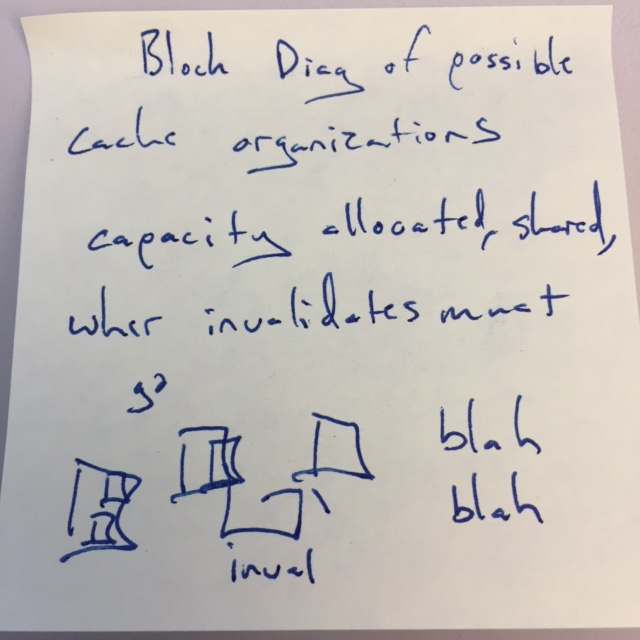
\includegraphics[width=0.9\columnwidth]{figures/cacheorg.jpg}
    \caption{Diagram showing potential cache organizations and effect on invalidations.}
    \label{fig:cacheorg}
\end{figure}



\begin{figure*}[tp]
    \centering
    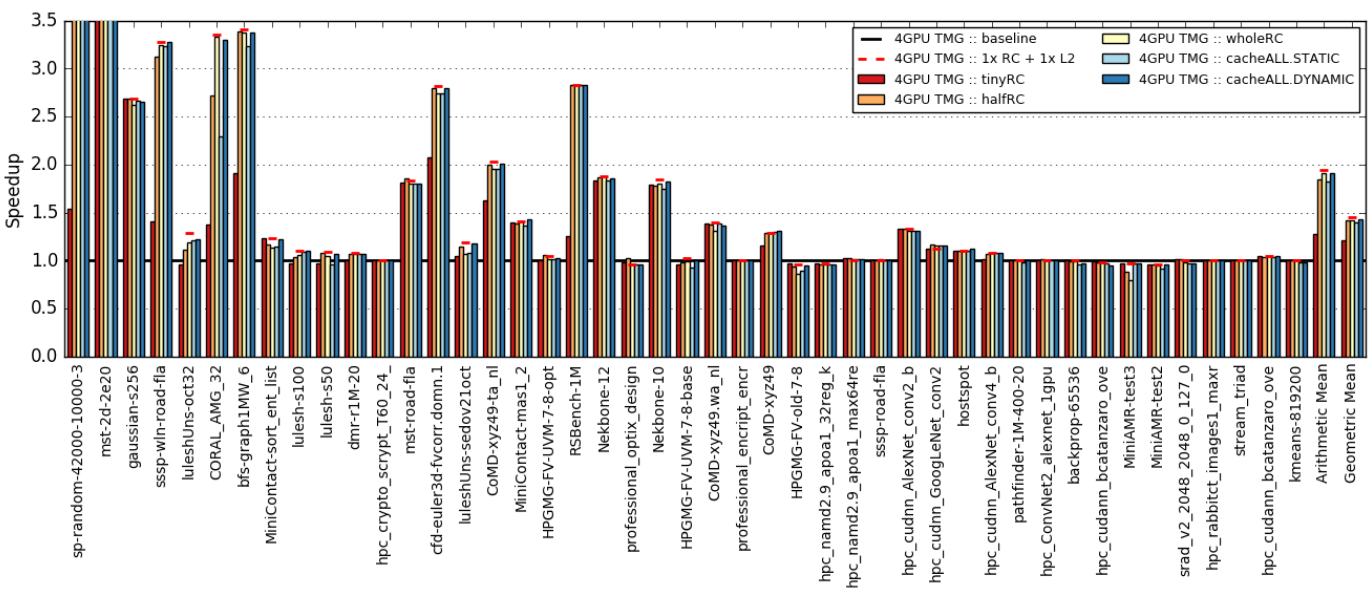
\includegraphics[width=0.9\textwidth]{figures/caching.jpg}
    \caption{Show one big plot with most of the data for various cache configurations.}
    \label{fig:caching}
\end{figure*}


\subsubsection{Results}
Results here

\begin{figure}[tp]
    \centering
    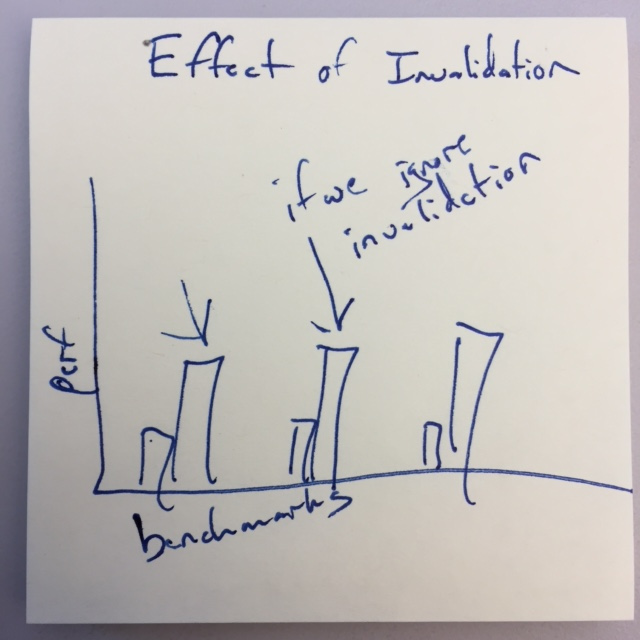
\includegraphics[width=0.9\columnwidth]{figures/invalidations.jpg}
    \caption{Show that cost of invalidations is still small at 4 GPUs.  Not unreasonable, but improved invalidations will matter in future.}
    \label{fig:invalidations}
\end{figure}


% \section{Results}
% \label{results}
% We evaluate the performance of selective GPU caching through iterative addition of our three proposed microarchitectural
% enhancements on top of naive selective caching. We then add promiscuous read-only caching and 
% finally present a sensitivity study for scenarios where the workload footprint is too large for a 
% performance-optimal page placement split across CPU and GPU memory.
% 
% \subsection{Microarchitectural Enhancements}
% Figure~\ref{fig:uncachableperformance} shows the baseline performance of naive selective caching
% compared to a hardware cache-coherent GPU.  Whereas performance remains as high as 95\% of the baseline 
% for some applications,
% the majority of applications suffer significant degradation, with applications like \texttt{btree}
% and \texttt{comd} seeing nearly an order-of-magnitude slowdown.  The applications that are hurt most
% by naive selective caching tend to be those that have a high L2 cache hit rate
% in a hardware cache-coherent GPU
% implementation like \texttt{comd} (Table~\ref{tab:gpuhitrate}) or those that are highly sensitive to L2 cache latency
% like \texttt{btree} (Figure~\ref{fig:cache_bw_latency}).  Prohibiting all GPU caching of CPU 
% memory results in significant over-subscription of the CPU
% memory system, which quickly becomes the bottleneck for application forward progress, resulting in
% nearly a 50\% performance degradation across our workload suite.
% 
% \begin{figure}[t]
% 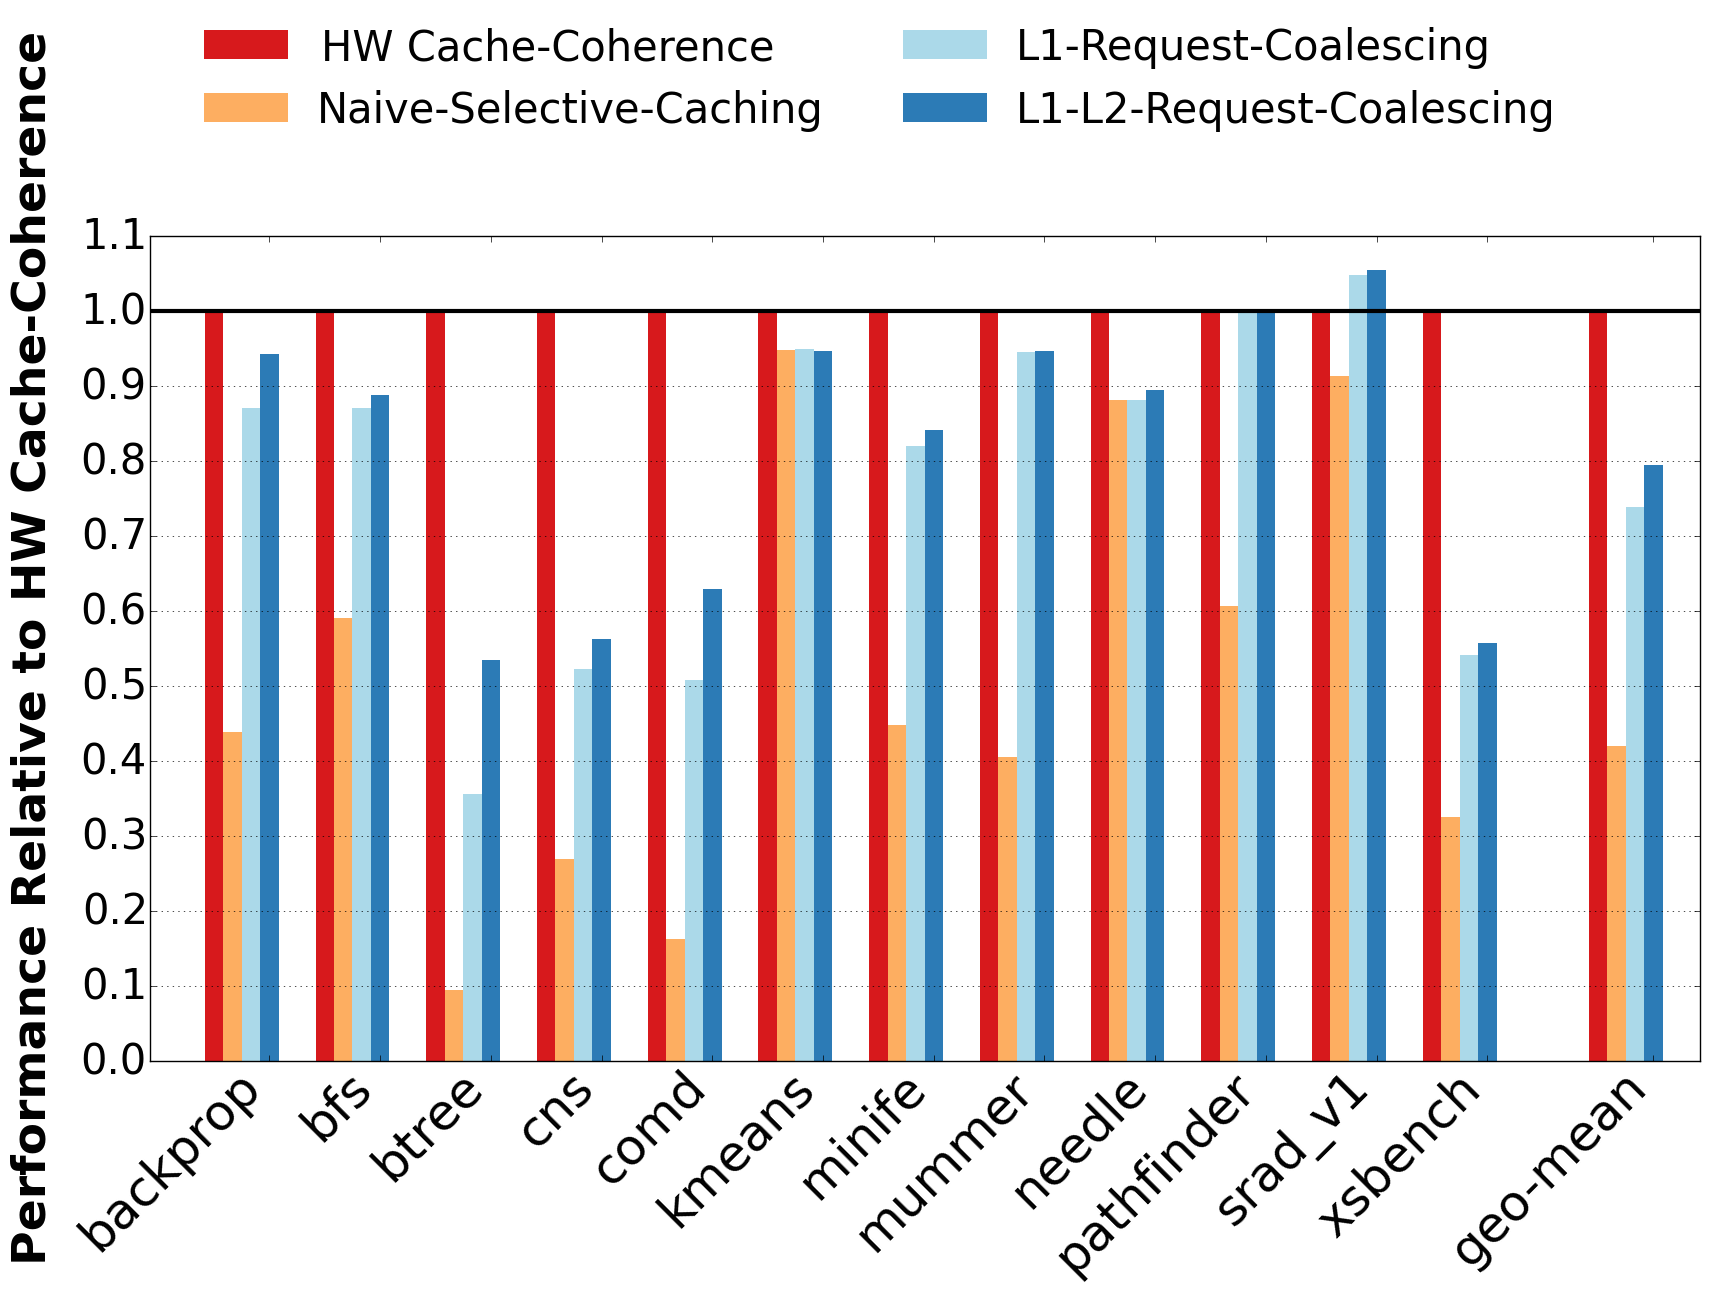
\includegraphics[width=1.0\columnwidth]{figures/unconstrainedperformance.png}
% \caption{GPU performance under selective caching with uncoalesced requests, L1 coalesced requests,
% L1+L2 coalesced requests.}
% \label{fig:uncachableperformance}
% \end{figure}
% 
% \subsubsection{Cacheless Request Coalescing}
% \label{mshrresults}
% Our first microarchitectural proposal is to implement cacheless request coalescing as described in Section~\ref{coalescing}.
% With naive selective caching relying on only the SIMD lane-level request coalescer within an SM, performance of the system degrades 
% to just 42\% of the hardware cache-coherent GPU, despite only 20\% of the application data residing in CPU physical memory.  
% Introducing request coalescing improves performance to 74\% and 79\% of a
% hardware cache-coherent GPU
% when using L1 coalescing and L1+L2 coalescing, respectively.  This improvement comes from
% a drastic reduction in the total number of requests issued across the CPU--GPU
% interconnect and reducing pressure on the CPU memory. Surprisingly \texttt{srad\_v1} shows
% a 5\% speedup over the hardware cache-coherent GPU when using L1+L2 request coalescing. \texttt{srad\_v1} has 
% a large number of pages
% that are written without first being read, thus the CPU DRAM system benefits from the elimination of reads that are caused
% by the write-allocate policy in the baseline GPU's L2 cache.
% Because the request coalescing hit rates, shown in
% Table~\ref{tab:coalescing_opportunity}, lag behind the hardware cached hit rates,
% selective caching still places a higher load on the interconnect and CPU memory
% than a hardware cache-coherent GPU, which translates
% into the 21\% performance reduction we observe when using selective caching with aggressive request coalescing.
% 
% \begin{figure}[t]
% 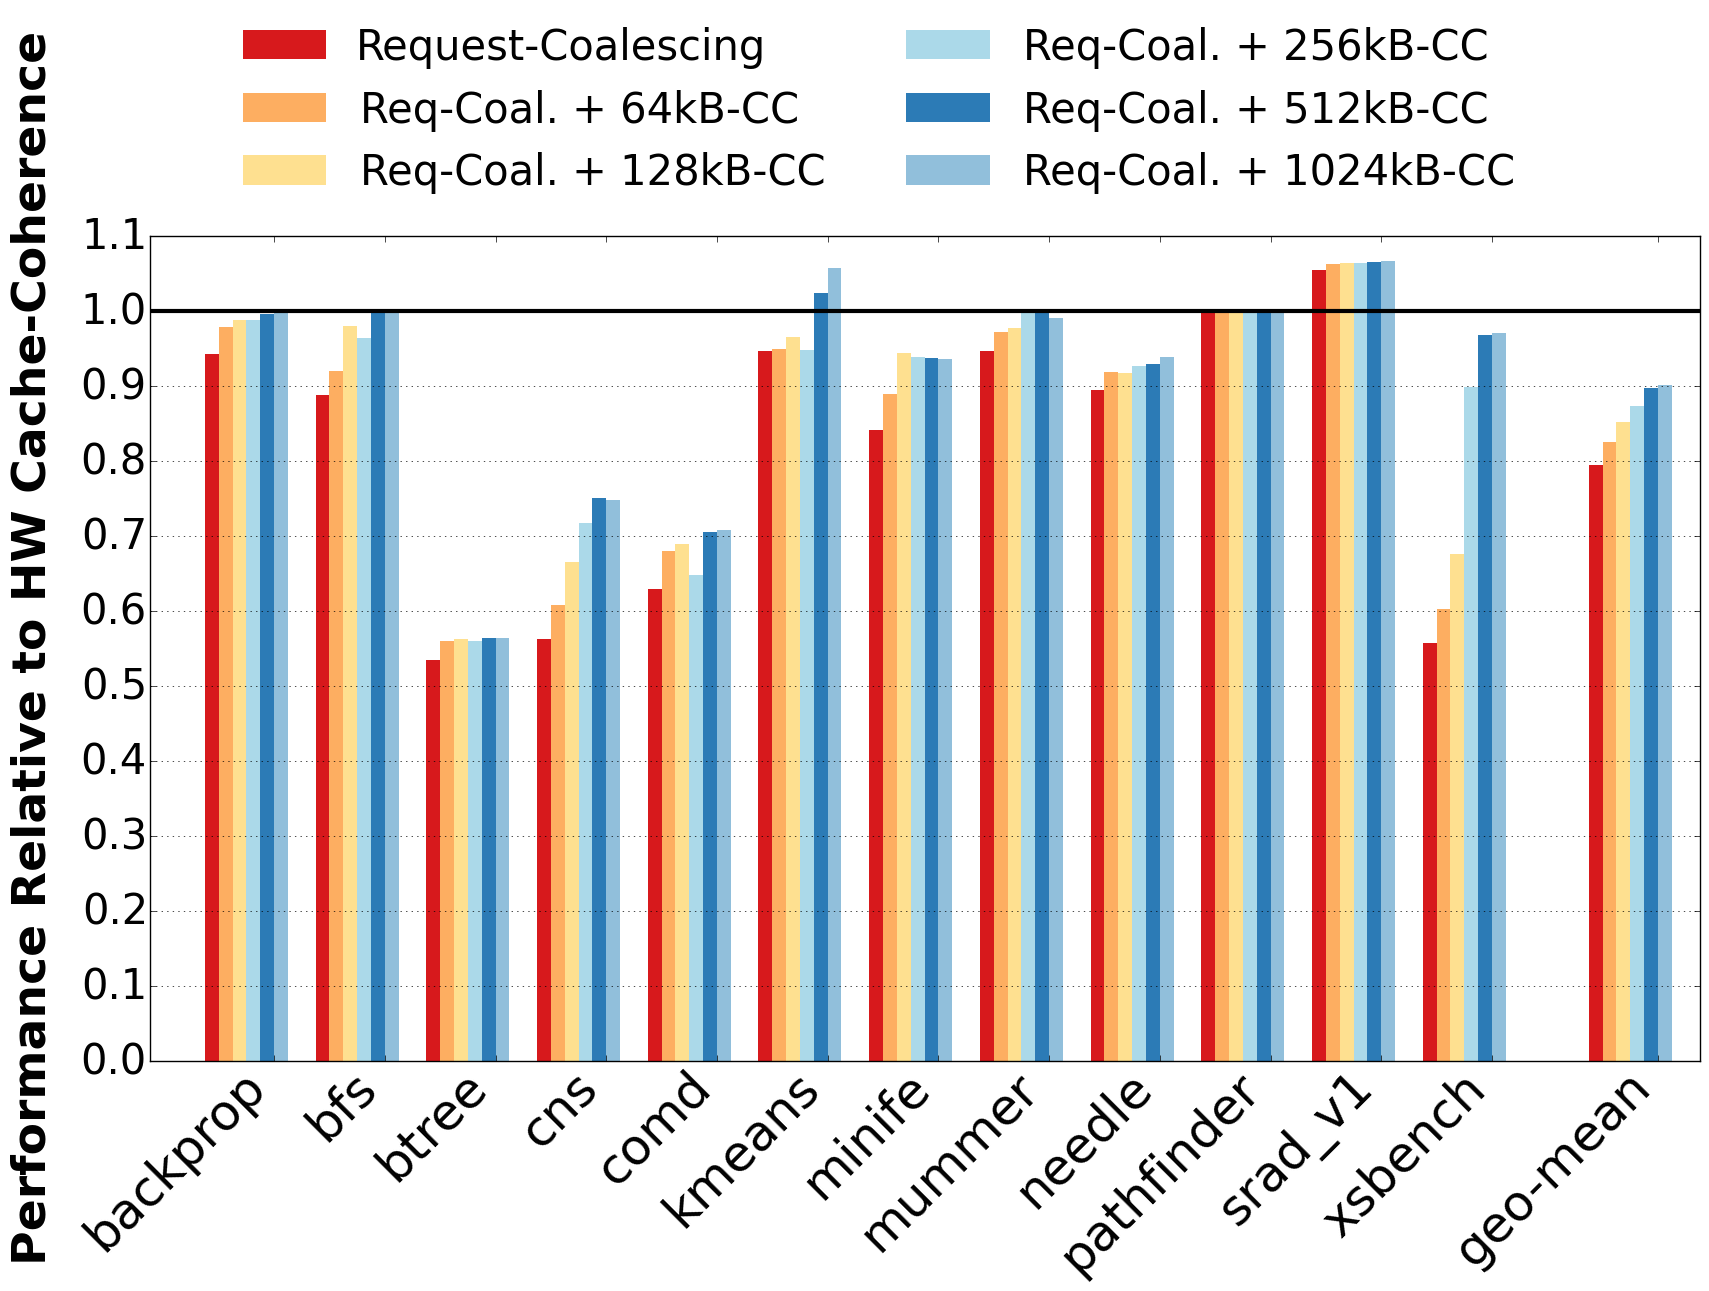
\includegraphics[width=1.0\columnwidth]{figures/unconstrainedperformanceMshrMCCache.png}
% \caption{GPU performance with selective caching when combining request coalescing with CPU-side
% caching for GPU clients at 64KB--1MB cache capacities. (CC: Client-Cache)}
% \label{fig:mccache}
% \end{figure}
% 
% \subsubsection{CPU-side Client Cache}
% \label{mccache}
% Whereas request coalescing captures much of the spatial locality provided by GPU L1 caches, it cannot capture
% any long distance temporal locality. Figure~\ref{fig:mccache} shows
% the performance differential of adding our proposed CPU-side client cache to L1+L2 request coalescing within the selective
% caching GPU. This GPU client cache not only reduces traffic to CPU DRAM from the GPU, but also improves latency for requests
% that hit in the cache and provides additional bandwidth that the CPU--GPU interconnect may exploit.  We observe
% that performance improvements scale with client cache size up to 512KB before returns diminish.  Combining
% a 512KB, 8-way associative client cache with request coalescing improves
% performance of our selective caching GPU to within 90\% of the performance of a
% hardware cache-coherent GPU\@. Note that \texttt{btree} only benefits marginally from
% this client cache because accessing the client cache still requires a round-trip interconnect
% latency of 200 cycles (Section~\ref{methodology}). \texttt{btree} is highly sensitive to
% average memory access latency (Figure~\ref{fig:cache_bw_latency}), which is not substantially improved by
% placing the client cache for GPU requests on the CPU die.
% 
% The size of an on-die CPU client cache is likely out of the hands of GPU architects, and
% for CPU architects allocating on-die resources for an external GPU client may seem an
% unlikely design choice.  However, this client cache constitutes only a small fraction of the
% total chip area of modern CPUs (0.7\% in 8-core Xeon E5~\cite{XeonLLC2013}) and is the size of just one additional private L2 cache
% within the IBM Power 8 processor.  Much like processors have moved towards on-die integration of PCIe to provide improved performance
% with external peripherals, we believe the performance improvements due to this cache are significant enough to warrant integration. 
% For CPU design teams, integrating such a cache into an existing design is likely easier than achieving performance by extending
% coherence protocols into externally developed GPUs. The GPU client cache also need not be specific to just GPU clients,
% other accelerators such as FPGAs or spatial architectures~\cite{Putnam2014,Parashar2013} that will be integrated along-side a traditional
% CPU architecture will also likely benefit from such a client cache.
% 
% \begin{figure}[t]
% 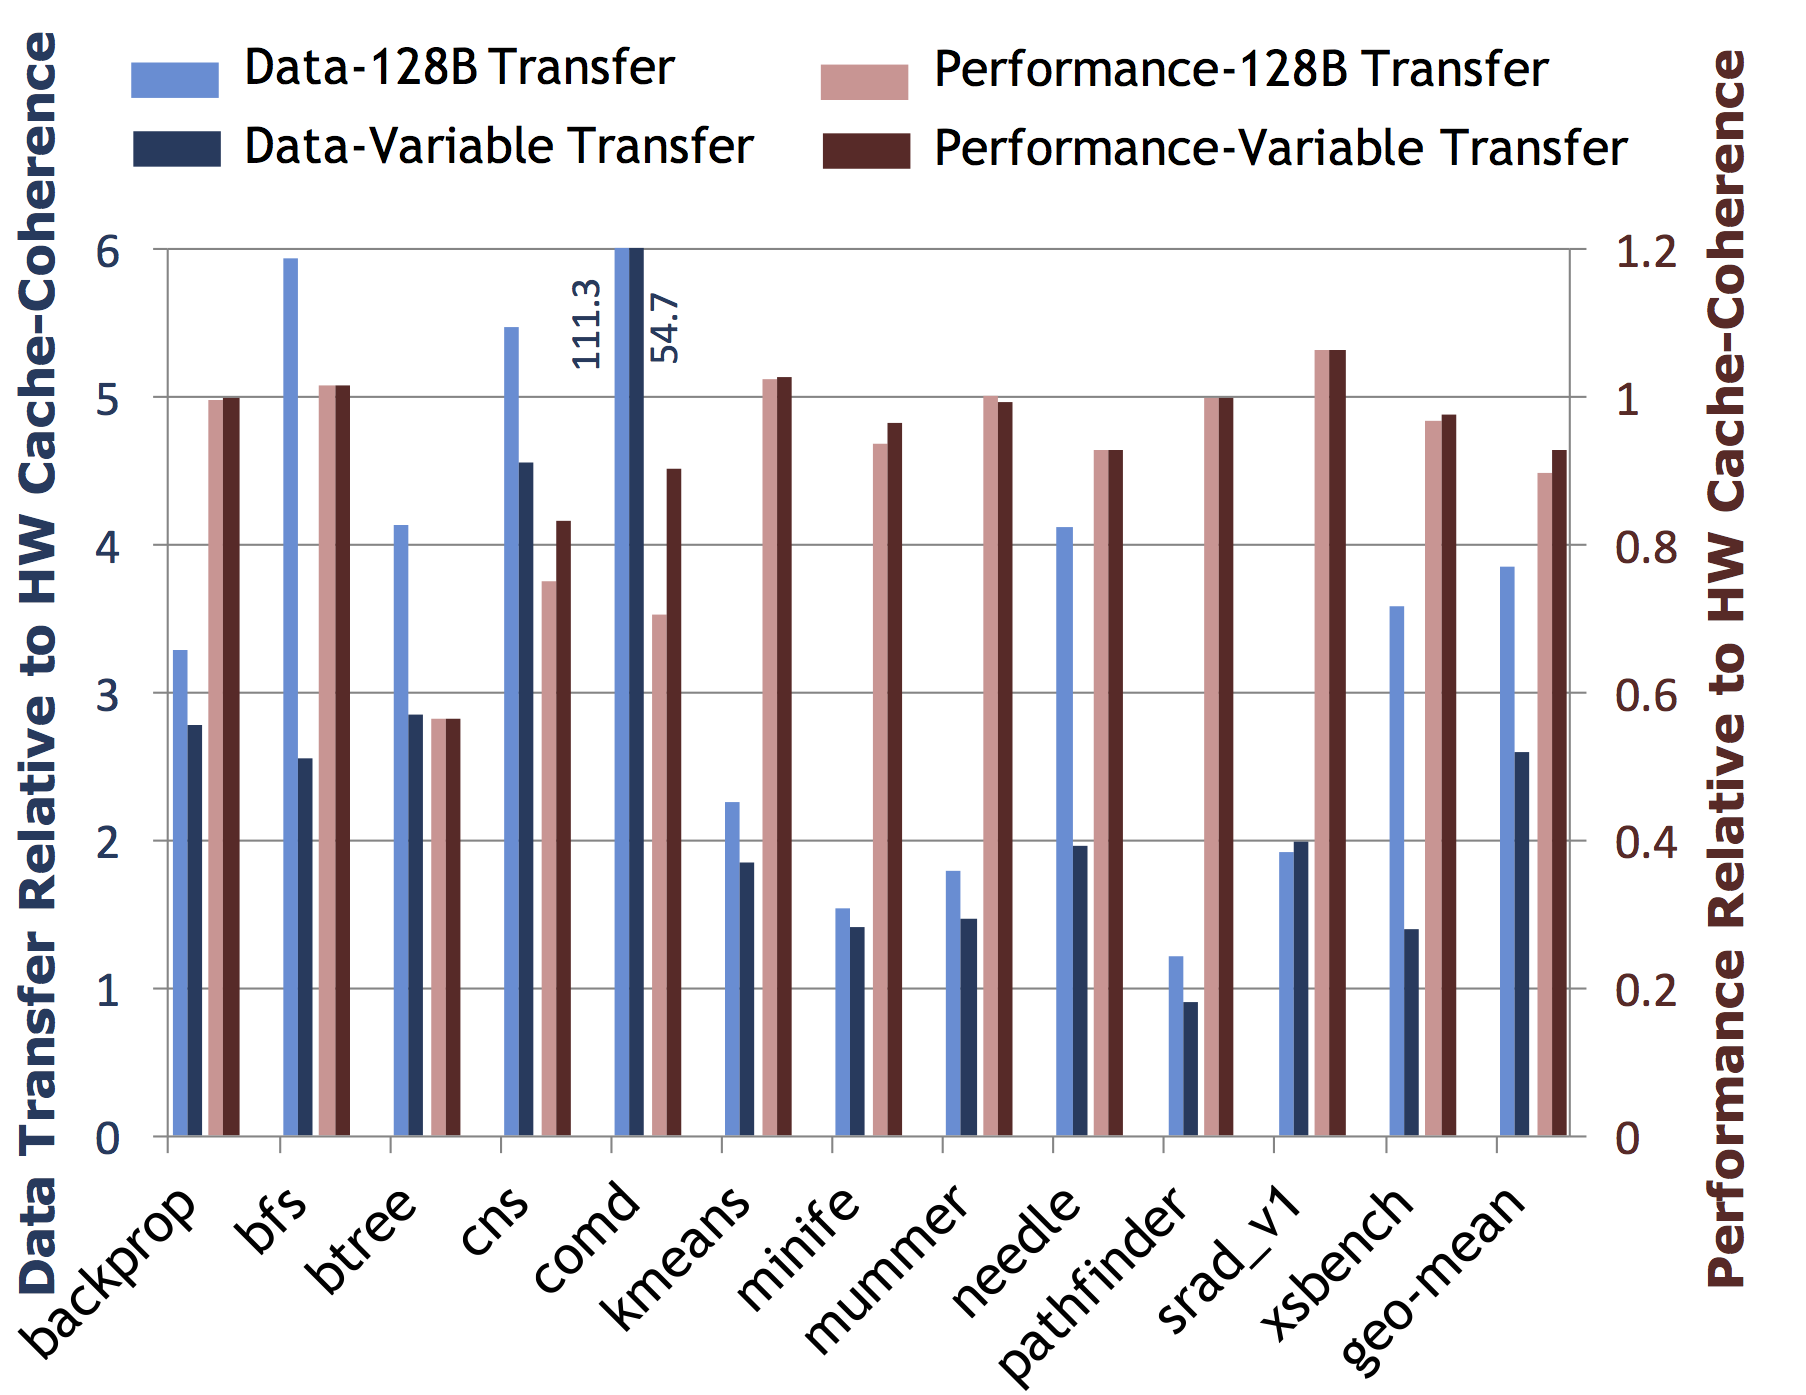
\includegraphics[width=1.0\columnwidth]{figures/linkimprovements.png}
% \caption{GPU data transferred across CPU-GPU interconnect (left y-axis) and performance (right y-axis)
% for 128B cache line-size link transfers and variable-size link transfers, respectively.}
% \label{fig:linkoptimization}
% \end{figure}
% 
% \begin{figure}[t]
% 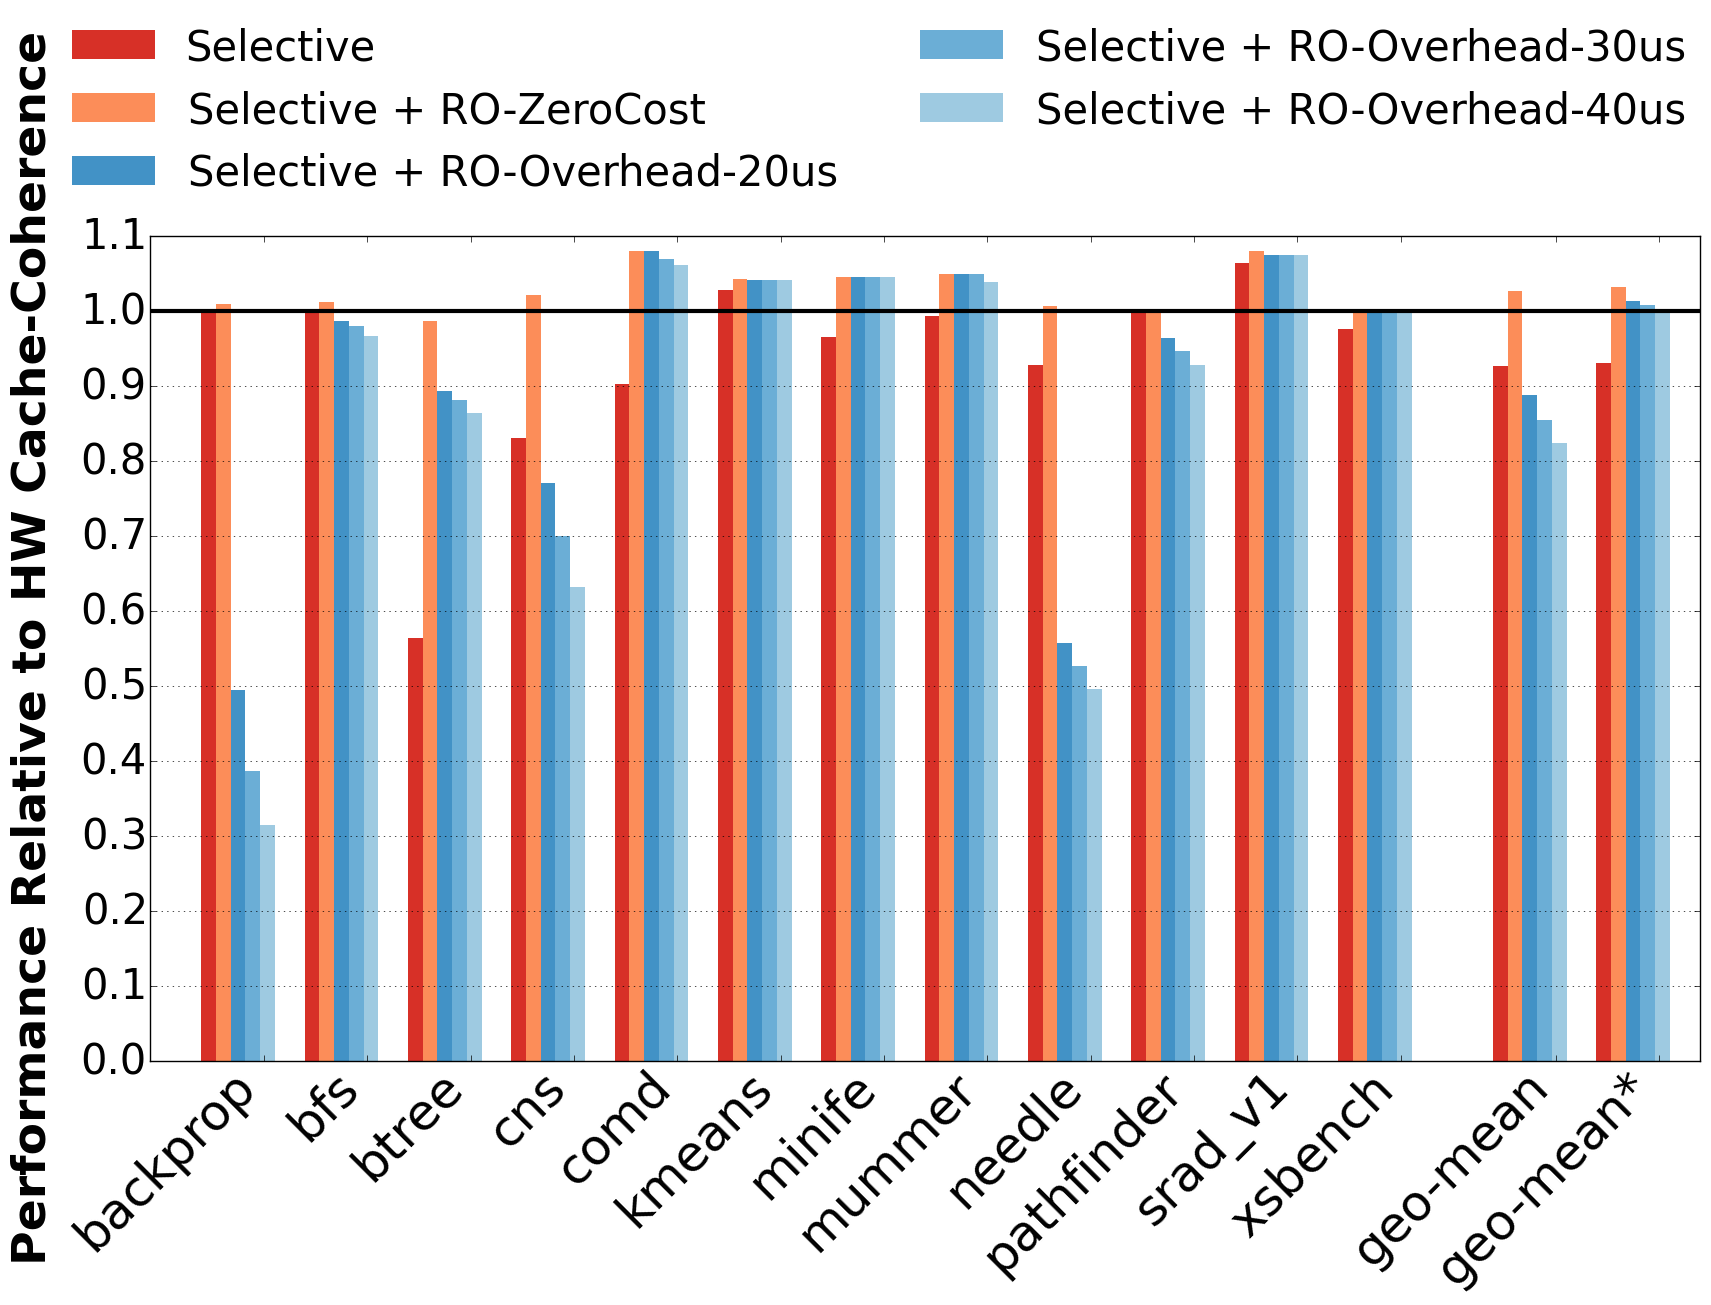
\includegraphics[width=1.0\columnwidth]{figures/readonlycaching.png}
% \caption{GPU performance when using Selective caching (Request-Coalescing +
% 512kB-CC + Variable-Transfers) combined with read-only
% caching. geo-mean*: Geometric mean excluding \texttt{backprop, cns,
% needle}, where read-only caching should be disabled. (RO: Read-Only)}
% \label{fig:readonlycaching}
% \vspace{-0.1in}
% \end{figure}
% 
% \subsubsection{Variable-size Link Transfers}
% \label{linkoptimization}
% Request coalescing combined with the CPU client cache effectively reduce the pressure on the CPU DRAM by limiting
% the number of redundant requests that are made to CPU memory.  The CPU client cache exploits temporal locality
% to offset data overfetch that occurs on the DRAM pins when transferring data at cache line granularity, but
% does not address CPU--GPU interconnect transfer inefficiency.
% To reduce this interconnect over-fetch, we propose variable-sized transfer units
% (see Section~\ref{variablesizing}). The leftmost two bars for each benchmark in Figure~\ref{fig:linkoptimization} show the total traffic across the
% CPU--GPU interconnect when using traditional fixed 128B cache line requests and
% variable-sized transfers, compared to a hardware cache-coherent
% GPU.  We see that despite request coalescing, our selective caching GPU transfers nearly 4 times the data
% across the CPU--GPU interconnect than the hardware cache-coherent GPU.  Our variable-sized transfer
% implementation reduces this overhead by nearly one third to just 2.6x more
% interconnect traffic than the hardware cache-coherent GPU.
% 
% This reduction in interconnect bandwidth results in performance gains of just
% 3\% on average, despite some applications like {\tt comd} showing significant improvements. 
% We observe that variable-sized transfers can significantly improve bandwidth utilization
% on the CPU--GPU interconnect but most applications remain performance-limited by the CPU memory 
% bandwidth, not the interconnect itself. When we increase interconnect bandwidth by 1.5x without enabling variable-sized
% requests, we see an average performance improvement of only 1\% across our benchmark suite.
% Variable-sized requests are not without value, however;
% transferring less data will save power or allow this expensive off-chip interface to be clocked at a lower
% frequency, but evaluating the effect of those improvements is beyond the scope of this work.
% 
% \subsection{Promiscuous GPU Caching}
% \label{readonlyresults}
% By augmenting selective caching with request coalescing, a GPU client cache, and variable-sized transfers,
% we achieve performance within 93\% of a hardware cache-coherent GPU\@. 
% As described in Section~\ref{readonly}, the GPU can be allowed to cache CPU memory that is contained
% within pages that are marked as read-only by the operating system. The benefit of caching data
% from such pages is offset by protection
% faults and software recovery if pages promiscuously marked as read-only 
% and cached by the GPU are later written.
% Figure~\ref{fig:readonlycaching} (RO-ZeroCost) shows the upper bound on possible improvements from read-only 
% caching for an idealized implementation that marks all pages as read-only and transitions them to
% read-write (and thus uncacheable)
% without incurring any cost when executing the required protection fault handling routine.  In a few cases, 
% this idealized implementation can outperform 
% the hardware cache-coherent GPU because of the elimination of write allocations in the GPU caches,
% which tend to have little to no reuse.
% 
% We next measure the impact of protection fault cost, varying the unloaded fault latency from
% 20us to 40us (see Figure~\ref{fig:readonlycaching}), commensurate with typical fault latencies on today's GPU implementations.
% While a fault is outstanding, the faulting warp and any other warp that accesses
% the same address are stalled; but, other warps may proceed, mitigating the impact of these faults on SM forward progress.  
% The latency of faults can be hidden if some warps executing on an SM are reading
% this or other pages.  However, if all warps issue writes at
% roughly the same time, the SM may stall due to a lack of schedulable warps or MSHR
% capacity to track pending faults. When accounting for fault overheads, 
% our selective caching GPU with promiscuous read-only caching achieves only 89\% of the performance of the 
% hardware cache-coherent GPU.
% 
% With a 20us fault latency, we see that 7 of 12 workloads 
% exhibit improvement from promiscuous read-only caching
% and that \texttt{btree} sees a large 35\% performance gain
% as it benefits from improvements to average memory
% access latency.
% In contrast, three workloads, \texttt{backprop}, \texttt{cns}, and
% \texttt{needle}, suffer considerable slowdowns due to the incurred protection fault latency.
% These workloads tend to issue many concurrent writes, exhausting the GPUs
% ability to overlap execution with the faults.  For such workloads, we advocate
% disabling promiscuous read-only caching in software (e.g., via a mechanism that tracks
% the rate of protection faults, disabling promiscuous read-only caching when the rate
% exceeds a threshold).
% 
% In summary, the effectiveness of promiscuous read-only caching depends heavily on
% the latency of protection faults and the GPU microarchitecture's ability to overlap the
% execution of non-faulting warps with those faults,
% which can vary substantially across both operating systems and architectures.  In
% systems where the fault latency is higher than the 20us (as measured on current NVIDIA systems), more
% judicious mechanisms must be used to identify read-only pages (e.g.,
% explicit hints from the programmer via the \texttt{mprotect} system call.)
